\section{Chameleon OpenStack}
\label{chameleon-openstack}
\index{Chameleon!Openstack}

OpenStack on Chameleon provides plenty of compute resources to
provision Linux virtual machines with various server types thus we can
deploy tools and software needed for the class and projects. This
hands-on tutorial is to walk through a basic step of getting access to
OpenStack Chameleon cloud under the class allocation and to provide
introduction to command line tools which are flexible and powerful
once it is mastered. Web interface, OpenStack Horizon is offered but
the class does not recommend to use it intensively because it has
limited to utilize cloud computing resources and it is difficult to
resolve issues when their are technical problems. Command line tools
generate full debugging messages if necessary.

\subsection{Account Creation}

The fist step to get access Chameleon cloud is to create a user
account if you do not already have one. You can skip to the next
section if you have a chameleon cloud account.

The register web page is available at:

\url{https://www.chameleoncloud.org/user/register/}

For more details, please als consult the chameleon chapter in the handbook.

\subsection{Join a Project}

The active project is required to use allocated compute resources to
the project.  Each class has a particular project number to use. Ask
details on Piazza, or instructor. Otherwise use the following
information to join a project:

\begin{lstlisting}
Spring 2018: CH-819337
\end{lstlisting}

The instructor (PI) will authorize you to join a project. Once you
have approved, you can start to launch a new VM instance on Chameleon
OpenStack.

\subsection{OpenStack RC File}

We will use Nova command line tools for Chameleon OpenStack and to
authorize our account on the command line tools, we need to obtain the
openstack RC file from the openstack web interface. Login to the
following page with your chameleon account:


\url{https://openstack.tacc.chameleoncloud.org/dashboard}

Confirm your project number and find \textbf{Access \& Security} on
the left menu.  The Access \& Security page has tabs and choose
\textbf{API Access} to download credentials on a local machine. Click
\textbf{Download OpenStack RC File} to download
\textit{CH-\$PROJECTID-openrc.sh} file on your machine.

  \begin{figure}[!htbp]
    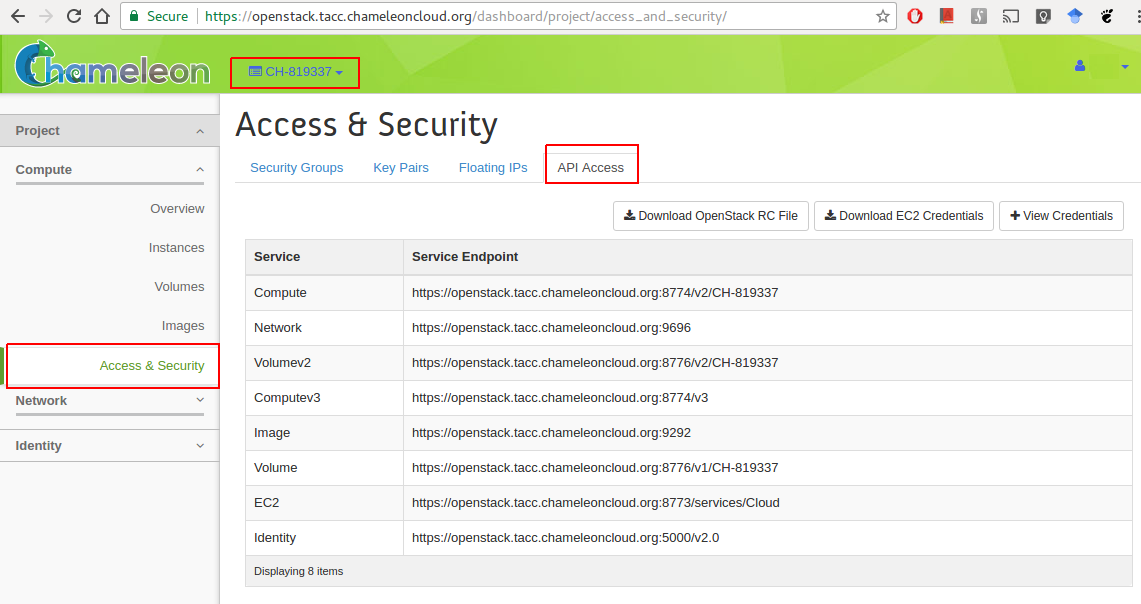
\includegraphics[width=8cm,height=8cm]{section/cloud/chameleon/images/openstack-chameleon-openrc.png}
    \centering
  \end{figure}

  This file contains REST API URLs that we use for Chameleon
  OpenStack.  Everytime you use nova command line tools, the file
  should be loaded on your terminal.

\begin{lstlisting}
mkdir ~/cloudmesh/chameleon
mv CH-\$PROJECTID-openrc.sh ~/cloudmesh/chameleon
source ~/cloudmesh/chameleon/CH-\$PROJECTID-openrc.sh
\end{lstlisting}

Once you \textit{source} the file, you can use nova command line tools
without sourcing it again.  The environment variables are enabled
while your terminal is alive.

\subsection{PIP Nova installation}

OpenStack provides \textit{nova} command line tools written by Python
which we will use in this tutorial. Run the following command to
install nova CLI on your machine.

\begin{lstlisting}
pip install python-openstackclient
\end{lstlisting}

Try nova command to see if it installed successfully:

\begin{lstlisting}
nova image-list
\end{lstlisting}

\begin{lstlisting}
\$ nova image-list
+--------------------------------------+--------------------------------------------------+--------+--------------------------------------+
| ID                                   | Name                                             | Status | Server                               |
+--------------------------------------+--------------------------------------------------+--------+--------------------------------------+
| be46bd5a-c4a5-4495-ad30-356186d8ff04 | CC-C7-autologin                                  | ACTIVE |                                      |
| 1fe5138b-300b-4b30-8d22-e728abbd7773 | CC-CentOS7                                       | ACTIVE |                                      |
...
\end{lstlisting}

The sample output messages look like above, if your installation is correctly
done.

\subsection{KeyPair Registration}

Once you have completed Nova CLI installation, SSH keypair registration is
required unless you already have one.

\begin{lstlisting}
nova keypair-add --pub-key \$HOME/ssh/id_rsa.pub \$USER-chameleon-key
\end{lstlisting}

Once you register your key, you can confirm the registration by:

\begin{lstlisting}
nova keypair-list
\end{lstlisting}

The sample output looks like:

\begin{lstlisting}
+----------------------+-------------------------------------------------+
| Name                 | Fingerprint                                     |
+----------------------+-------------------------------------------------+
| albert-chameleon-key | cf:04:06:aa:8b:76:af:77:aa:0a:b5:87:ff:0f:ba:97 |
+----------------------+-------------------------------------------------+
\end{lstlisting}

Note that if you do not have an existing SSH keypair, you can create
one by: and go back to the keypair registration step above to complete
the registration on OpenStack.

\begin{lstlisting}
ssh-keygen -t rsa -C \$USER-chameleon-key
\end{lstlisting}


\subsection{Start a new VM instance}

The \textit{nova boot} simple command will start a VM instance with
some parameters to specify which base image and a server size we will
use with a name. We use \textit{CC-Ubuntu16.04} base image in this
tutorial which is an official Ubuntu 16.04 image provided by Chameleon
project.

\begin{lstlisting}
nova boot --image CC-Ubuntu16.04 --key-name \$USER-chameleon-key --flavor m1.small \$USER-myfirst-instance
\end{lstlisting}

\subsection{Floating IP Address}

If your new VM instance is up and running, it needs external ip
address (floating IP address) to get access from your local
machine. The new instance only has an internal IP address as a
default. We will associate a floating IP address here to get SSH
access to a VM instance.

\begin{lstlisting}
 nova floating-ip-create ext-net
 +--------------------------------------+----------------+-----------+----------+---------+
 | Id                                   | IP             | Server Id | Fixed IP | Pool    |
 +--------------------------------------+----------------+-----------+----------+---------+
 | 13dc309e-9a82-45af-8a9a-7fbd74f4aec6 | 129.114.111.37 | -         | -        | ext-net |
 +--------------------------------------+----------------+-----------+----------+---------+
\end{lstlisting}

Now we have a IP address to assign to a VM instance. In this tutorial,
we will associate \textit{129.114.111.37} to our
\$USER-myfirst-instance VM instance by:

\begin{lstlisting}
nova floating-ip-associate \$USER-myfirst-instance 129.114.111.37
\end{lstlisting}

Once you completed this step, you are now able to SSH into your VM
instance.  Confirm \textit{ACTIVE} state in your VM to get access.

\begin{lstlisting}
| f19e0ba1-9b76-46f4-896f-378983ab2aa3 | albert-myfirst-instance       | ACTIVE  | -          | Running     | CH-819337-net=192.168.0.13, 129.114.111.37 |
\end{lstlisting}


\begin{lstlisting}
ssh cc@129.114.111.37
\end{lstlisting}

Note that \textit{cc} is login name your your VM if you start a VM
with the official Chameleon cloud image.

\subsection{Termination of VM Instance}

If you completed your work on your VM instance, you have to terminate
your VM and release a floating IP address associated with. For
example, we terminate our first instance and the IP address by:

\begin{lstlisting}
nova delete \$USER-myfirst-intance
nova floating-ip-delete 129.114.111.37
\end{lstlisting}


